%=========================================================================
% (c) 2011, 2012 Josef Lusticky

\section{Clock library extension}\label{sec:design-clock}
The previous section described how the call for getting the time acquires
the maximum precision the clock model allows.
Section~\ref{sec:analysis-time} showed that there can be unpredictable
results caused by a race condition when reading the {\it{scount}} variable
and the counter register {\it{TCNT2}} afterwards.
Although the read could be wrapped with an interrupt disable,
the common solution on AVR platform in Contiki is to perform more read operations,
compare the results and perform read operations again if the results are not consistent.
Figure~\ref{fig:design-read} shows such a solution.

\begin{figure}
  \centering
  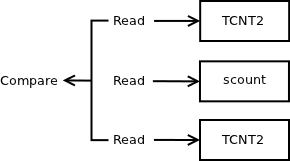
\includegraphics[width=6cm,keepaspectratio]{fig/read.png}
  \caption{Multiple read and result comparison}
  \label{fig:design-read}
\end{figure}

The call for adjusting the time computes the number of clock ticks
with the longer or shorter tick interval.
For storing the result, a new variable must be introduced.
If the value of this variable is zero, no adjustments are in progress.
Otherwise, the default value of the compare register is incremented or decremented by 1
and written to {\it{OCR2A}}.
This effectively causes adjusting the time, as described in section~\ref{sec:analysis-interface}.
When the time was adjusted enough,
the default value of the compare register is written back to {\it{OCR2A}}.

Section~\ref{sec:analysis-clock-interface} explained, that the default value
of the compare register for AVR Raven in Contiki is 31,
but the number of counter register increments between two successive interrupts is 32.
Incrementing the compare register value causes one real second to be experienced as
$\frac{f_{T2}}{CLOCK\_SECOND \times (32 + 1)} = \frac{4096}{128~\times~33} = 0.\overline{96}$~seconds
by the operating system.
Decrementing the compare register value causes one real second to be experienced as
$\frac{f_{T2}}{CLOCK\_SECOND \times (32 - 1)} = \frac{4096}{128~\times~31} \doteq 1.032258$~seconds
by the operating system.

Each increment of the counter register {\it{TCNT2}} takes
$\frac{1}{128 \times 32} = 0.000244140625$~seconds.
This is also the minimal possible clock adjustment,
that can be achieved by changing the compare register value just for one clock tick.
The fastest possible adjustment is approximately 0.03~$\frac{s}{s}$.
If faster adjustments were needed, the compare register would have to be updated with different values. 
However, updating the compare register with more different values would require
a more complicated software design
and lower values could cause a miss of the compare match as described in section~\ref{sec:analysis-hwclock}.

% TO NTP INTERFACE
%When writing to compare register, the value is transferred to a
%temporary register, and latched after two positive edges of a source clock~\cite{avr-datasheet}.
%The user should not write a new value before the contents
%of the temporary register have been transferred to its destination.
%To detect that a transfer to the destination register has taken place,
%the Asynchronous Status Register - ASSR has been implemented.
%Since writing to compare register occurs only once within interrupt CONTEXT, % context?
%this detection is not mandatory.
